\chapter{静态电磁场及其边值问题的解}

\section{静电场基本方程}
理想导体的$E_2$、$D_2$、$H_2$、$B_2$均为0,故有:
$$\left\{
\begin{aligned}
\nabla \times \vec{E} = 0 &\qquad\text{理想导体表面上的}\vec{E}\text{的切向分量为0}\\
\nabla \cdot \vec{D} = \rho_S&\qquad\text{理想导体表面上的电荷密度等于}\vec{D}\text{的法向分量}
\end{aligned}
\right.$$
积分形式:
$$\left\{
\begin{aligned}
\oint_C \vec{E} \cdot \mathrm{d}\vec{l} = 0\\
\oint_S \vec{D} \cdot \mathrm{d}\vec{S} = q
\end{aligned}
\right.$$
本构关系:
$$D = \varepsilon E$$

\section{静电场边界条件}
$$\left\{
\begin{aligned}
	\vec{e}_n \times (\vec{E}_1 - \vec{E}_2) = 0 \\
	\vec{e}_n \cdot (\vec{D}_1 - \vec{D}_2) = \rho_S
\end{aligned}
\right.$$
若分界面的电荷为0,则$\rho_S = 0$。

\section{场矢量的折射关系}
\begin{figure}[h]
	\centering
	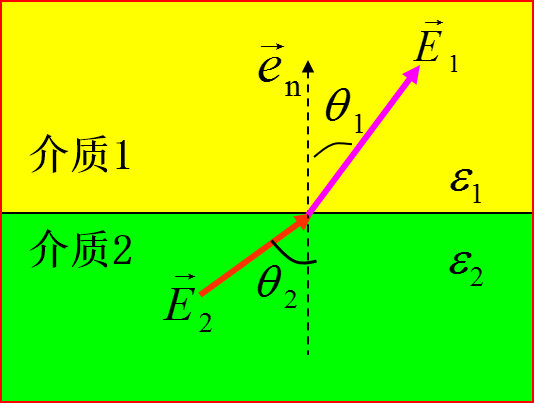
\includegraphics[keepaspectratio]{pics/场矢量折射关系}
	\caption{场矢量折射关系}
	\label{fig:fieldrefraction}
\end{figure}
$${{\tan {\theta _1}} \over {\tan {\theta _2}}} = {{{E_{{\rm{1t}}}}/{E_{{\rm{1n}}}}} \over {{E_{{\rm{2t}}}}/{E_{{\rm{2n}}}}}} = {{{\varepsilon _{\rm{1}}}/{D_{{\rm{1n}}}}} \over {{\varepsilon _{\rm{2}}}/{D_{{\rm{2n}}}}}} = {{{\varepsilon _1}} \over {{\varepsilon _2}}}$$


\section{导体表面的边界条件}
在静电平衡的情况下,导体内部的电场为0,则导体表面的边界条件为:
$$\left\{
\begin{aligned}
\vec{e}_n \times \vec{E} = 0 \\
\vec{e}_n \cdot \vec{D} = \rho_S
\end{aligned}
\right.$$

\section{电位函数}
\subsection*{电位函数}
静电场可以用一个标量函数的梯度来表示,标量函数$\phi$称为静电场的标量电位或简称电位。
$$\nabla \times \vec{E} = 0 \Rightarrow \vec{E} = -\nabla\phi$$

\subsection*{电位}
连续体分布电荷电位:
$$\phi(\vec{r}) = \frac{1}{4\pi\varepsilon} \int_V \frac{\rho(\overrightarrow{r}')}{R}\mathrm{d}V' + C$$
其中,$C$为积分操作时产生的常数。

面电荷电位:
$$\phi(\vec{r}) = \frac{1}{4\pi\varepsilon} \int_S \frac{\rho_S(\overrightarrow{r}')}{R}\mathrm{d}S' + C$$

线电荷电位:
$$\phi(\vec{r}) = \frac{1}{4\pi\varepsilon} \int_l \frac{\rho_l(\overrightarrow{r}')}{R}\mathrm{d}l' + C$$

点电荷电位:
$$\phi(\vec{r}) = \frac{1}{4\pi\varepsilon R} + C$$

\subsection*{电位差}
电场力做功(将单位正电荷从$P$移向$Q$)等于$P$、$Q$两点之间的电位差:
$$\int_P^Q E  \cdot {\rm{d}}\vec l =  - \int_P^Q {{\rm{d}}\phi }  = \phi (P) - \phi (Q)$$

\section{电位的微分方程(泊松与拉普拉斯方程)}
在均匀介质中,有泊松方程:
$$\nabla^2 \phi = -\frac{\rho}{\varepsilon}$$
在无源区域,因为$\rho = 0$,所以有:
$$\nabla^2 \phi = 0$$

\section{静电位的边界条件}
设$P_1$和$P_2$是介质分界面两侧紧贴界面的相邻两点,其电位分别为$\phi_1$和$\phi_2$。当两点间距离$\Delta l \to 0$时,$\phi_1 = \phi_2$。

$$\left\{
\begin{gathered}
\vec{e}_n \cdot (\vec{D_1} - \vec{D_2}) = \rho_S \\
\vec{D} = -\varepsilon\nabla\phi
\end{gathered}
\right. \Rightarrow {\varepsilon _2}{{\partial {\phi _2}} \over {\partial n}} - {\varepsilon _1}{{\partial {\phi _1}} \over {\partial n}} = {\rho _S}$$

若介质分界面上无自由电荷,即$\rho_S = 0$,则:
$${\varepsilon _2}{{\partial {\phi _2}} \over {\partial n}} = {\varepsilon _1}{{\partial {\phi _1}} \over {\partial n}}$$

导体表面上电位的边界条件($\phi$为常数):$$\varepsilon {{\partial \phi } \over {\partial n}} =  - {\rho _S}$$

\section{电容}
孤立导体的电容定义为所带电量$q$与其电位$\phi$的比值,即
$$C = \frac{q}{\phi}$$
电容的大小只与导体系统的几何尺寸、形状和及周围电介质的特性参数有关,而与导体的带电量和电位无关。

\subsection*{计算电容的一般方法}
\begin{enumerate}
	\item 假定两导体上分别带电荷$+q$和$-q$;
	\item 计算两导体间的电场强度$E$;
	\item 由由$U = \int^2_1\vec{E}\cdot\mathrm{d}\vec{l}$,求出导体间的电位差;
	\item 用比值法$C = \frac{q}{U}$求解电容。
\end{enumerate}

\section{静电场的能量和能量密度}
\subsection*{静电场能量}
$${W_{\rm{e}}} = {1 \over 2}q\phi $$
$${\rm{d}}{W_{\rm{e}}} = {1 \over 2}\rho \phi {\rm{d}}V$$
体分布电荷的电场能量:
$${W_{\rm{e}}} = {1 \over 2}\int_V {\rho \phi {\rm{d}}V} $$
面分布电荷的电场能量:
$${W_{\rm{e}}} = {1 \over 2}\int_S {{\rho _S}\phi {\rm{d}}S} $$

\subsection*{静电场的能量密度}
电场能量密度:
$${w_{\rm{e}}} = {1 \over 2}\vec D \cdot \vec E$$

静电场的总能量:
$${W_{\rm{e}}} = {1 \over 2}\int_V {\vec D \cdot \vec E{\rm{d}}V} $$

对于线性、各向同性介质,则有:
$${w_{\rm{e}}} = {1 \over 2}\vec D \cdot \vec E = {1 \over 2}\varepsilon \vec E \cdot \vec E = {1 \over 2}\varepsilon {E^2}$$
$${W_{\rm{e}}} = {1 \over 2}\int_V {\vec D \cdot \vec E{\rm{d}}V}  = {1 \over 2}\int_V {\varepsilon \vec E \cdot \vec E{\rm{d}}V}  = {1 \over 2}\int_V {\varepsilon {E^2}{\rm{d}}V} $$

推证:
$$W_e = {1 \over 2}\oint_S {\phi \vec D \cdot {\rm{d}}\vec S + } {1 \over 2}\int_V {\vec E \cdot \vec D{\rm{d}}V} $$

\section{恒定电场基本方程及边界条件}
\subsection*{恒定电场基本方程}
微分形式:
$$\left\{
\begin{aligned}
	\nabla \cdot \vec{J} = 0 \\
	\nabla\times\vec{E} = 0
\end{aligned}
 \right.$$

积分形式:
$$\left\{
\begin{aligned}
	\oint_S\vec{J}\cdot\mathrm{d}\vec{S} = 0 \\
	\oint_C\vec{E}\cdot\mathrm{d}\vec{l} = 0
\end{aligned}
\right.$$

线性各向同性导电媒质的本构关系:
$$\vec{J} = \sigma\vec{E}$$

若媒质是均匀的,则:
$$\nabla  \cdot {\vec J} = \nabla  \cdot (\sigma \vec E) = \sigma \nabla  \cdot \vec E = 0 \Rightarrow \nabla\cdot\vec{E} = 0$$

恒定电场的电位函数:
$$\nabla  \times {\vec E} = 0 \Rightarrow \vec E =  - \nabla \phi $$
$$\nabla  \cdot {\vec J} = 0 \Rightarrow \nabla  \cdot (\sigma \nabla \phi ) = 0\Rightarrow{\nabla ^2}\phi = 0$$

\subsection*{恒定电场的边界条件}
场矢量的边界条件:
$$\oint_S {{\vec J}}  \cdot {\rm{d}}{\vec S} = 0 \Rightarrow {\vec e_{\rm{n}}} \cdot ({{\vec J}_1} - {{\vec J}_2}) = 0 \Rightarrow {J_{1{\rm{n}}}} = {J_{{\rm{2n}}}}$$
$$\oint_C {{\kern 1pt} {\vec E}}  \cdot {\rm{d}}{\vec l} = 0 \Rightarrow {\vec e_{\rm{n}}} \times ({{\vec E}_1} - {{\vec E}_2}) = 0 \Rightarrow {E_{{\rm{1t}}}} = {E_{{\rm{2t}}}}$$

场矢量的折射关系,图\ref{fig:steadyelecfieldfraction}:
\begin{figure}[h]
	\centering
	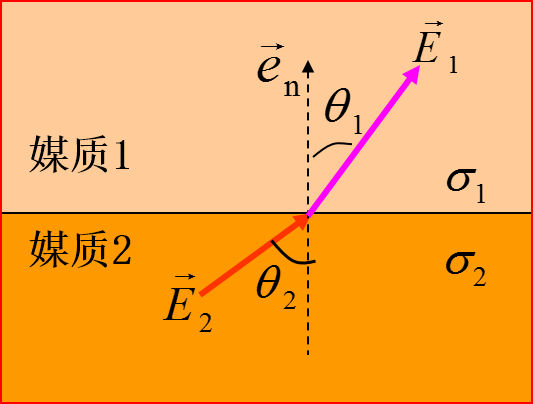
\includegraphics[keepaspectratio]{pics/恒定电场的场矢量折射关系}
	\caption{恒定电场的场矢量折射关系}
	\label{fig:steadyelecfieldfraction}
\end{figure}

$${{\tan {\theta _1}} \over {\tan {\theta _2}}} = {{{E_{{\rm{1t}}}}/{E_{{\rm{1n}}}}} \over {{E_{{\rm{2t}}}}/{E_{{\rm{2n}}}}}} = {{{\sigma _{\rm{1}}}/{J_{{\rm{1n}}}}} \over {{\sigma _{\rm{2}}}/{J_{{\rm{2n}}}}}} = {{{\sigma _1}} \over {{\sigma _2}}}$$

导电媒质分界面上的电荷面密度:
$$ \rho_S = \overrightarrow{e_n} \cdot (\vec{D_1} - \vec{D_2}) = \overrightarrow{e_n}\cdot (\frac{\varepsilon_1}{\sigma_1}\vec{J_1} - \frac{\varepsilon_2}{\sigma_2}\vec{J_2}) = (\frac{\varepsilon_1}{\sigma_1} - \frac{\varepsilon_2}{\sigma_2})J_n $$

电位的边界条件:
$${\phi _1} = {\phi _2},\quad {\sigma _1}{{\partial {\phi _1}} \over {\partial n}} = {\sigma _2}{{\partial {\phi _2}} \over {\partial n}}$$

\textbf{注:}恒定电场同时存在于导体内部和外部,在导体表面上的电场既有法向分量又有切向分量,电场并不垂直于导体表面,因而导体表面不是等位面。


\section{恒定电场与静电场的比拟(图\ref{fig:assimilation})}
PS:吐个槽,因为公式太多懒得画表格,就从PPT里面直接另存为图片的。不得不说,MathType的公式真$\cdot$吃藕。也可能是写公式的人比较懒吧。
\begin{figure}[h]
	\centering
	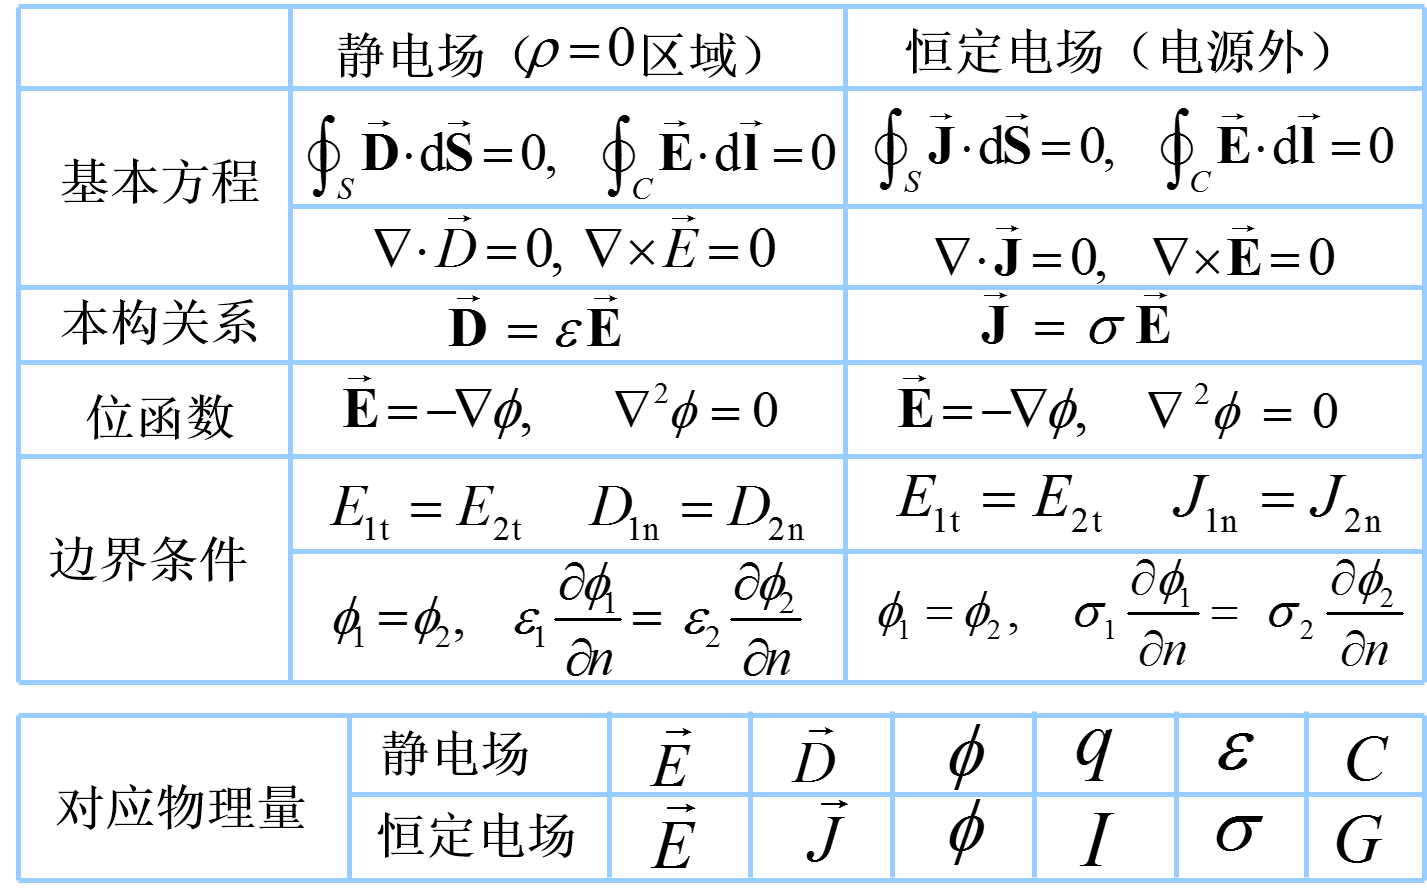
\includegraphics[width=\linewidth]{pics/恒定电场与静电场的比拟}
	\caption{恒定电场与静电场的比拟}
	\label{fig:assimilation}
\end{figure}

\section{漏电导}
漏电流与电压之比为漏电导,即:
$$G = {I \over U}$$

其倒数称为绝缘电阻,即:
$$R = {1 \over G} = {U \over I}$$

\subsection*{计算电导的方法}
\subsubsection*{法一}
\begin{enumerate}
	\item 假定两电极间的电流为$I$;
	\item 计算两电极间的电流密度矢量$\vec{J}$;
	\item 由$J = \sigma E$得到$E$;
	\item 由$U = \int^2_1\vec{E}\cdot\mathrm{d}\vec{l}$,求出两导体间的电位差。
	\item 求比值$G = \frac{I}{U}$,即得出所求电导。
\end{enumerate}

\subsubsection*{法二}
\begin{enumerate}
	\item 假定两电极间的电位差为$U$;
	\item 计算两电极间的电位分布$\varphi$;
	\item 由$\vec{E} = -\nabla\phi$得到$\vec{E}$;
	\item 由$J = \sigma E$得到$J$。
	\item 由$I = \int_S \vec{J}\cdot\mathrm{d}\vec{S}$,求出两导体间电流。
	\item 求比值$G = \frac{I}{U}$,即得出所求电导。
\end{enumerate}

\subsubsection*{法三}
经典比拟法:
$${G \over C} = {\sigma  \over \varepsilon }$$

\section{恒定磁场的基本方程和边界条件}
\subsection*{恒定磁场的基本方程}
微分形式:
\[\left\{ \begin{gathered}
\nabla  \times \vec H = \vec J \hfill \\
\nabla  \cdot \vec B = 0 \hfill \\ 
\end{gathered}  \right.\]

积分形式:
\[\left\{ \begin{gathered}
\oint_C {{\kern 1pt} \vec H}  \cdot d\vec l = \int_S {{\kern 1pt} \vec J \cdot d\vec S}  \hfill \\
\oint_S {{\kern 1pt} \vec B}  \cdot d\vec S = 0 \hfill \\ 
\end{gathered}  \right.\]

本构关系:
\[\vec B = \mu \vec H\]

\subsection*{恒定磁场的边界条件}
边界条件方程:
\[\left\{ \begin{gathered}
{{\vec e}_{\text{n}}} \cdot ({{\vec B}_1} - {{\vec B}_2}) = 0 \hfill \\
{{\vec e}_{\text{n}}} \times ({{\vec H}_1} - {{\vec H}_2}) = {{\vec J}_S} \hfill \\ 
\end{gathered}  \right.\]

若分界面上不存在面电流,即$J_S = 0$,则:
\[\left\{ \begin{gathered}
{{\vec e}_{\text{n}}} \cdot ({{\vec B}_1} - {{\vec B}_2}) = 0 \hfill \\
{{\vec e}_{\text{n}}} \times ({{\vec H}_1} - {{\vec H}_2}) = 0 \hfill \\ 
\end{gathered}  \right.\]

\section{恒定磁场的矢量磁位}
恒定磁场可以用一个矢量函数的旋度来表示:
\[\nabla  \cdot \vec B = 0 \Rightarrow \vec B = \nabla  \times \vec A\]

\subsection*{库仑规范}
与电位一样,磁矢位也不是惟一确定的,它加上任意一个标量$\varPsi$的梯度以后,仍然表示同一个磁场:
\[\vec A' = \vec A + \nabla \psi \Rightarrow \nabla  \times \vec A' = \nabla  \times \vec A + \nabla  \times (\nabla \psi ) = \nabla  \times \vec A\]
其中,$\vec{A}$为矢量磁位或称磁矢位
磁矢位的任意性是因为只规定了它的旋度,没有规定其散度造成的。为了得到确定的A,可以对A的散度加以限制,在恒定磁场中通常规定    ,并称为库仑规范。

\subsection*{磁矢位方程}
微分方程:
\[\left.
\begin{aligned}
	\vec{B} = \nabla \times \vec{A} \\
	\nabla \times \vec{B} = \mu \vec{J}
\end{aligned}
\right\} \Rightarrow \nabla \times \nabla \times \vec{A} = \mu \vec{J} \Rightarrow \nabla (\nabla \cdot \vec{A}) - \nabla^2\vec{A} = \mu \vec{J}\]

矢量泊松方程:
\[ \nabla \cdot \vec{A} = 0 \Rightarrow \nabla^2 \vec{A} = -\mu\vec{J} \]

无源区$\vec{J} = 0$时,有矢量拉普拉斯方程:
\[ \nabla^2 \vec{A} = 0 \]

\subsection*{磁矢位的表达式}
\[\nabla  \times (\frac{{\vec J(\vec r')}}
{R}{\text{)}} = \vec J(\vec r') \times \nabla (\frac{1}
{R}{\text{)}} - \frac{1}
{R}\nabla  \times \vec J(\vec r') = \vec J(\vec r') \times \nabla (\frac{1}
{R}{\text{)}} \Rightarrow \vec{A'}(\vec{r'}) = \frac{\mu}{4\pi} \int_V \frac{\vec{J'}(\vec{r'})}{R} \mathrm{d}V' \]

面电流磁矢位:
\[ \vec{A'}(\vec{r'}) = \frac{\mu}{4\pi} \int_S \frac{\vec{J'}(\vec{r'})}{R} \mathrm{d}S' \]

细线电流磁矢位:
\[ \vec{A'}(\vec{r'}) = \frac{\mu}{4\pi} \int_C \frac{\vec{J'}(\vec{r'})}{R} \mathrm{d}\vec{l'} \]

利用磁矢位计算磁通量:
\[\Phi  = \int_{{\kern 1pt} S} {\,\vec B \cdot {\text{d}}\vec S}  = \int_{{\kern 1pt} S} {\,\nabla  \times \vec A \cdot {\text{d}}\vec S}  = \oint_{{\kern 1pt} C} {{\kern 1pt} \vec A \cdot {\text{d}}\vec l} \]

磁矢位的边界条件:
\[\left.
\begin{aligned}
\oint \vec{A}\cdot\mathrm{d}\vec{l} = \int_S \vec{B}\cdot\mathrm{d}\vec{S} \Rightarrow A_{1t} = A_{2t} \\
\nabla \cdot \vec{A} = 0 \Rightarrow \oint_S\vec{A}\cdot\mathrm{d}\vec{S} = 0 \Rightarrow A_{1n} = A_{2n}
\end{aligned}
\right\} \Rightarrow \vec{A_1} = \vec{A_2} \]

\[\left.
\begin{aligned}
\vec{e_n} \times (\vec{H_1} - \vec{H_2}) = \vec{J_S} \\
\vec{H} = \nabla \times \frac{\vec{A}}{\mu}
\end{aligned}
\right\} \Rightarrow \vec{e_n} \times ( \frac{1}{\mu_1}\nabla\times\vec{A_1} -  \frac{1}{\mu_2}\nabla\times\vec{A_2}) = \vec{J_S} \]

\section{恒定磁场的标量磁位}
标量磁位或磁标位:
\[\vec H =  - \nabla {\varphi _{\text{m}}}\]
即在无传导电流(J=0)的空间中,可以引入一个标量位函数来描述磁场。

磁标位的微分方程:
\[\nabla  \cdot \vec B = 0,\vec B = {\mu _0}(\vec H + \vec M) \Rightarrow \nabla  \cdot \vec H =  - \nabla  \cdot \vec M = \frac{{{\rho _{\text{m}}}}}{{{\mu _0}}}\]
其中,等效磁荷体密度:
\[{\rho _{\text{m}}} =  - {\mu _0}\nabla  \cdot \vec M\]

将\(\vec H =  - \nabla {\varphi _{\text{m}}}\)代入\(\nabla  \cdot \vec H = \frac{{{\rho _{\text{m}}}}}{{{\mu _0}}}\)
得:
\[{\nabla ^2}{\varphi _{\text{m}}} =  - \frac{{{\rho _{\text{m}}}}}
{{{\mu _0}}}\]

在线性、各向同性的均匀媒质中:
\[{\nabla ^2}{\varphi _{\text{m}}} = 0\]

\subsection*{标量磁位的表达式}
与静电位比较,有:
\[\varphi (\vec r) = \frac{1}{4\pi\varepsilon_0}\int_V \frac{\rho (\vec r')}{R} \mathrm{d}V'\Rightarrow\varphi_\text{m}(\vec r) = \frac{1}{4\pi\mu_0}\int_V {\frac{\rho _\text{m}(\vec r')}{R}} \text{d}V'\]

\subsection*{标量磁位的边界条件}
\[\varphi_{m1} = \varphi_{m2}, \quad{\mu _1}\frac{{\partial {\varphi _{{\text{m1}}}}}}
{{\partial n}} = {\mu _2}\frac{{\partial {\varphi _{{\text{m2}}}}}}
{{\partial n}}\]
或:
\[\varphi_{m1} = \varphi_{m2}, \quad\frac{{\partial {\varphi _{m2}}}}
{{\partial n}} - \frac{{\partial {\varphi _{{\text{m1}}}}}}
{{\partial n}} =  - \frac{{{\rho _{{\text{m}}S}}}}
{{{\mu _0}}}\]
其中,有等效磁荷面密度:
\[{\rho _{{\text{m}}S}} =  - {\mu _0}{\vec e_{\text{n}}}\cdot({\vec M_2} - {\vec M_1})\]

\section{磁标位与静电位的比较(图\ref{fig:magneticeleccompare})}
\begin{figure}[h]
	\centering
	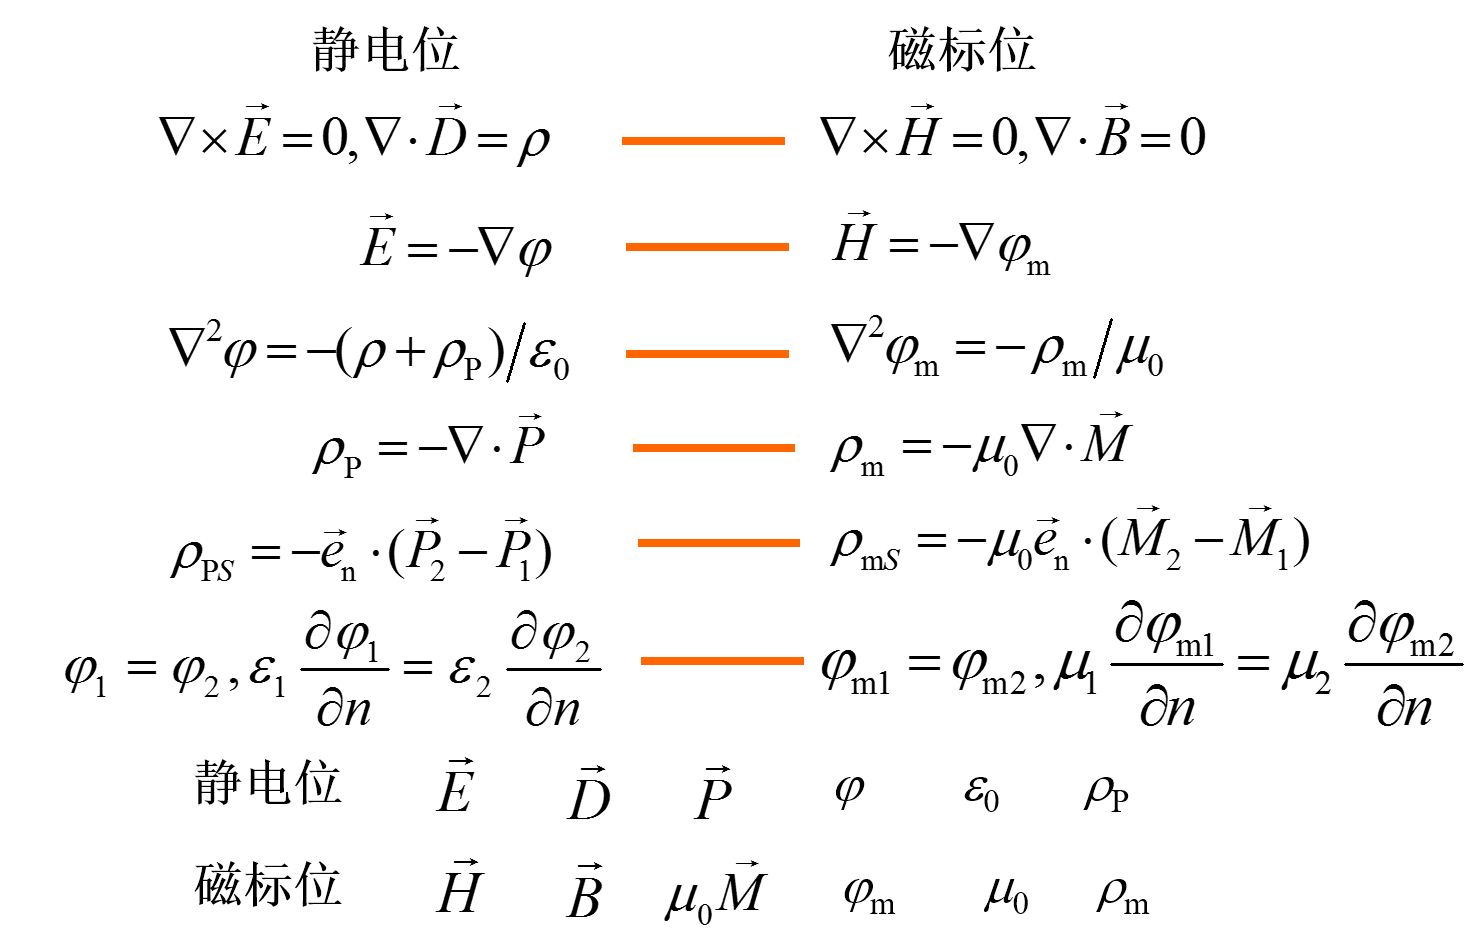
\includegraphics[width=\linewidth]{pics/磁标位与静电位的比较}
	\caption{磁标位与静电位的比较}
	\label{fig:magneticeleccompare}
\end{figure}

\section{磁通量}
单匝线圈形成的回路的磁链定义为穿过该回路的磁通量:
\[ \varPsi = \varPhi \]

多匝线圈形成的导线回路的磁链定义为所有线圈的磁通总和:
\[\Psi  = \sum_i {{\Phi _i}} \]

\section{自感}
设回路$C$中的电流为$ I $,所产生的磁场与回路$ C $交链的磁链为$ \varPsi $,则磁链$ \varPsi $与回路$ C $中的电流$ I $有正比关系,其比值
\[L = \frac{\Psi}{I}\]
称为回路 C 的自感系数,简称自感。

粗导体回路的自感:
\[ L = L_i + L_o \]
其中,$L_i = \frac{\Psi_i}{I}$为内自感,$L_o = \frac{\Psi_o}{I}$为外自感。

\section{恒定磁场的能量}















